% SPDX-License-Identifier: Apache-2.0
\documentclass[11pt,a4paper]{article}
\usepackage[margin=23mm,headheight=15pt]{geometry}
\usepackage[T1]{fontenc}
\usepackage[utf8]{inputenc}
\usepackage{lmodern,microtype,amsmath,amssymb,booktabs,tabularx,longtable,array}
\usepackage{graphicx,xcolor,enumitem,fancyhdr,titlesec}
\usepackage[unicode,hidelinks]{hyperref}
\usepackage{xurl}
\definecolor{cosmic}{HTML}{251343}
\definecolor{cyan}{HTML}{087E8B}
\definecolor{gold}{HTML}{A47019}
\definecolor{muted}{HTML}{4D5667}
\hypersetup{colorlinks=true,linkcolor=cosmic,urlcolor=cyan,citecolor=cyan,pdftitle={AGI ALPHA: Game-Theoretic Discovery of Productive Advantage},pdfauthor={AGI ALPHA / MontrealAI}}
\titleformat{\section}{\Large\bfseries\color{cosmic}}{\thesection}{0.7em}{}
\titleformat{\subsection}{\large\bfseries\color{cosmic}}{\thesubsection}{0.7em}{}
\setlist{nosep,leftmargin=1.5em}
\setlength{\parskip}{5pt}
\setlength{\parindent}{0pt}
\setlength{\emergencystretch}{3em}
\pagestyle{fancy}
\fancyhf{}
\fancyhead[L]{\small\color{muted}AGI ALPHA \enspace / \enspace PRODUCTIVE TRANSFER}
\fancyhead[R]{\small\color{muted}26 October 2026}
\fancyfoot[L]{\small\color{muted}Reproducible research \textperiodcentered\ bounded claims}
\fancyfoot[R]{\small\thepage}
\renewcommand{\headrulewidth}{0.3pt}
\newcommand{\artifact}[1]{\texttt{\small\path{#1}}}
\newcommand{\B}{\textsf{B}}
\newcommand{\Ctwo}{\textsf{C2}}
\begin{document}
\hypersetup{pageanchor=false}
\begin{titlepage}
\thispagestyle{empty}
\vspace*{12mm}
{\large\bfseries\color{cyan}AGI ALPHA FLYWHEEL}\par
\vspace{8mm}
{\Huge\bfseries\color{cosmic}Game-Theoretic Discovery\\of Productive Advantage}\par
\vspace{6mm}
{\LARGE From Transferred Capabilities to Financeable Growth}\par
\vspace{8mm}
{\large SUCCESSOR $\Omega$ Harness \enspace $\cdot$ \enspace Transformational Intelligence}\par
\vspace{6mm}
{AGI ALPHA / MontrealAI \hfill 26 October 2026}\par
\vspace{9mm}
{\small
\textbf{Abstract.}
We test whether external research can improve useful production and finance the same retained capability inside AGI ALPHA. A DUPLEX-inspired model-extraction stage feeds the unchanged source verifier and SUCCESSOR Workbench. The first six-task campaign yields complete inventories but no complete customer handoffs; its conventional comparator also imposed an unfair proof requirement. Those failures are preserved. A separately frozen four-task follow-up accepts all A/B customer reports and three of four C2 reports. C2 adds two out-of-scope data operations; B matches the incumbent's required conclusions. Actual complete costs remain unknown. The planned 166-cell three-arm market campaign is gated, not narrowed. A separately registered A/B negative control executes 384 enterprise histories: zero investment, zero incremental B profit, and twelve profitable worlds per arm. These are conditional implementation checks, not demand validation. We demonstrate functional source-intake transfer, but no identified incremental economic advantage or commercial Flywheel.

\medskip
\textbf{Résumé.}
Nous testons si une méthode externe améliore un travail utile et finance la capacité réellement évaluée dans AGI ALPHA. L’extraction inspirée de DUPLEX alimente le vérificateur et le Workbench inchangés. Le premier essai conserve ses échecs de livraison et de comparaison. Sur quatre nouvelles tâches figées, A et B produisent quatre rapports acceptés; C2 en produit trois et ajoute deux opérations hors périmètre. B égale les conclusions de la référence. Les coûts complets restent inconnus. Les 166 scénarios à trois bras demeurent bloqués. Un diagnostic A/B distinct exécute 384 historiques d’entreprise : aucun investissement, aucun profit incrémental de B, douze mondes rentables par bras. Ce transfert fonctionnel ne démontre ni avantage économique identifié, ni Flywheel commercial modélisé complet, ni réussite commerciale réelle.
}

\vfill
\begin{minipage}{0.96\textwidth}
\color{muted}\small
\textbf{Evidence identity.} Study \texttt{AGI-ALPHA-PRODUCTIVE-TRANSFER-20261026-v1}.
The original primary campaign, its unsuccessful conventional implementation and incomplete customer packages are preserved. A separately registered follow-up uses fresh inputs. Monetary scenarios are conditional simulations, not observed sales. Actual customer collections are zero.
\par\medskip
\textbf{Companion.} Executable source, prospective freezes, source and license records, raw model responses, unchanged product and Workbench snapshots, independent acceptance, resource ledgers, full new market histories and a bilingual offline demonstration accompany this paper. Earlier publications remain independently owned and unchanged.
\end{minipage}
\end{titlepage}
\hypersetup{pageanchor=true}

\section{The question is useful work, then finance}
A retained capability becomes economically meaningful only when it improves an outcome that a buyer has reason to accept. A promising architecture is not evidence of that improvement. The mechanism tested here is: useful work worth buying, profitable delivery, justified capability investment, better fresh work, and resources for another worthwhile improvement. Each arrow requires its own evidence. We distinguish four levels throughout:
\begin{enumerate}
\item \textbf{Engineering transfer}: a reproducible benefit on fresh work in the actual AGI ALPHA system.
\item \textbf{Economic improvement}: benefits exceed the complete incremental investment over a defensible workload.
\item \textbf{Modeled commercial Flywheel}: an evidence-grounded market model finances the actual tested asset from collected operating resources; its benefits support a further justified investment.
\item \textbf{Realized commercial Flywheel}: actual accepted work, collections and reconciled costs establish that cycle outside simulation.
\end{enumerate}
The first level does not imply the second, and a positive simulated cash balance does not establish either a realized market or a second worthwhile capability. Self-acceleration would additionally require evidence that the process of constructing capabilities itself improves; this experiment does not supply that evidence.

Our offering is a bounded dependency-maintenance decision. A maintainer supplies a public consumer scope and two captured dependency versions. The deliverable identifies every relevant call in that scope, links exact source evidence, checks supported argument binding, states material uncertainty, and gives a practical next action in English and French. A conflict can justify holding an upgrade and revising a named call. Preserved argument binding can narrow the investigation, but cannot certify behavior, imports, types, security or release readiness. An unresolved call must name the missing evidence and the test or inspection needed next.

This is an actual maintenance question rather than an API inventory. It is also narrower than complete dependency qualification. Dependabot and Renovate already provide free or community alternatives for parts of update discovery and pull-request creation; a competent maintainer can combine them with source search and existing tests. Neither their availability nor our execution establishes willingness to pay for this particular bounded review \cite{dependabot,renovate}.

\section{Starting from the real system}
\subsection{Source, ownership and retained boundaries}
We inspected all four requested repositories and coordinated through issue 4850 \cite{coordination}. At the recorded checkpoint, Alpha main was \texttt{a8b057068717}; Fleet was \texttt{45759fb096fa}; AGIJobs was \texttt{bc4abbd5c28f}; and AGIJobManager was \texttt{5d5670df9dbb}. Complete identities and read receipts are in the source register. These are distinct repositories and authority surfaces, not interchangeable components of a synthetic benchmark.

The executed product is the public source-only upgrade-decision implementation at commit \texttt{97057bd2bf21}; its core SHA-256 begins \texttt{6cf46d13a2a4}. The native Workbench is an unchanged nine-file source closure at commit \texttt{eb07086ac427}, including the actual \texttt{createWorkbench(adapters)} implementation. Our finite adapter adds a mission family; it does not recreate the engine. Every run preserves HOLD admission, empty authority, disconnected settlement and unauthenticated local history. No held native execution path is promoted to operator approval. Existing runtime and publication owners remain responsible for their own lanes.

A local product-owner checkout contained two unpublished fixes and differed from the public snapshot. We retained the failed identity comparison and rejected that local candidate for this study. The public snapshot was then frozen. This matters: favorable local code must not silently replace the declared incumbent. Existing useful-work and game-theoretic publications are preserved separately, including their negative results and exploratory diagnostics.

Verified token roles remain distinct. The inspected AGIJobManager source uses USDC with six decimals for its settlement configuration; AGIJobs uses the separate AGIALPHA token interface with eighteen decimals. The study executes neither payment path. No token issuance, customer savings, valuation, treasury balance or nominal token quantity is booked as operating profit. No new contract or financial transaction is part of the experiment.

\subsection{Audit of the previous strategic-market result}
A fresh arithmetic auditor reconciled all 19,440 original enterprise histories, including every cash movement, bill and invoice, reserve and obligation, rejected-delivery revenue rule, and decision-time financing check. Nine selected arm executions were replayed exactly. The original market core's SHA-256 is recorded in the companion. The auditor is a separate same-session implementation; it is not independent institutional replication.

\begin{table}[htbp]
\centering\small
\begin{tabularx}{\textwidth}{Xrrrr}
\toprule
Preserved campaign & Worlds & Enterprises & Investments & Earned-funded\\
\midrule
Primary & 2,088 & 6,264 & 0 & 0\\
Exploratory sensitivities & 2,472 & 7,416 & 12 & 0\\
Fixed-price diagnostic & 1,920 & 5,760 & 796 & 0\\
\bottomrule
\end{tabularx}
\caption{The previous negative conclusion remains intact. Every exploratory or diagnostic investment was seed-funded. ``Earned-funded'' means investment from available collected operating surplus, not initial capital or unpaid invoices.}
\end{table}

The original primary failure cannot be read as a clean experiment showing that all demand is insufficient. A later diagnostic identified a materially unhelpful pricing heuristic that repeatedly proposed high, unbought prices. A fixed-price diagnostic produced some profitable cases and more seed-funded adoption, but still no earned-funded investment. That diagnostic does not overwrite the primary result or justify tuning price against the same confirmation set.

Other binding uncertainties remain: customer value, alternatives, trust and switching effort, delivery and construction costs, utilization, cash timing and reserves. The historical model did not identify them from observed buyers. A better extractor can remove a production step while leaving every one of these commercial obstacles binding.

\subsection{Measured production burden}
The earlier 61-case target observer took a median 15.231 seconds of wall time and 0.217 seconds of CPU. Its mandatory timeout check took about 15.016 seconds, or 98.6\% of wall time. Removing that check would change the acceptance boundary, not demonstrate productive transfer. No executable-search framework was installed to optimize this already understood wait.

The observed intake burden was different. The product consumes a curator-authored \texttt{alpha-upgrade-call-request/v1}: exact consumer call locations and before/after declaration selectors with captured source bodies. Its existing core already performs deterministic checks and a second binding verification using Python's \texttt{inspect.Signature.bind}. The missing stage is turning a raw consumer/dependency package into that precise request. This is the intervention point studied here.

\section{External ideas as hypotheses}
\begin{table}[htbp]
\centering\small
\begin{tabularx}{\textwidth}{p{25mm}XX}
\toprule
Source & What was learned & What was actually evaluated\\
\midrule
Virtual Agent Economies & Strategic allocation, interaction and resource constraints. & Conceptual support for the inherited behavioral market. No imported demand calibration or equilibrium guarantee.\\
DUPLEX & Model extraction into a structured representation; deterministic tools perform exact work. & A source-intake adaptation feeding the existing verifier. No reproduction of its robot, PDDL or planning benchmark.\\
OpenEvolve & Bounded executable search with charged proposals, failures and evaluations. & Source/version/license audit. Not installed or evaluated: no justified expensive repeated executable target was identified.\\
EnvHarness & Failure-targeted environment construction with fresh acceptance outside the training loop. & Source/version/license audit. No environment-learning claim; synthetic controls repair implementation defects, and fresh sources remain held out.\\
\bottomrule
\end{tabularx}
\caption{Reading a method and evaluating its transfer are separate activities. Only the structured-extraction principle was adapted into the production experiment.}
\end{table}

Virtual Agent Economies is a conceptual foundation for resource-constrained agent interaction, not a substitute for buyer evidence \cite{vae}. DUPLEX reports a pipeline involving model extraction, scripted planning representations, an exact planner and bounded repair; its published domains and repeated evaluations differ substantially from dependency maintenance \cite{duplex}. In particular, repeated household trials are not hundreds of independent customer tasks. We do not import its reported success rates, latencies or cost gains.

The inspected OpenEvolve repository was version 0.4.0 at head \texttt{66856ac4ba2f}, Apache-2.0, with Python 3.10 or later and dependencies including OpenAI, PyYAML, NumPy, tqdm, Flask, dacite and cloudpickle. The inspected EnvHarness package was 0.0.1 at \texttt{fab7d57441f0}, Apache-2.0, requiring Python 3.10 or later and including Pydantic, PyYAML and LiteLLM. Its README model tables and default configuration require separate attention; a reported benchmark model is not automatically the installed default \cite{openevolve,envharness}. Exact source bodies, licenses, versions, evaluation notes and limitations are retained. No author-linked DUPLEX implementation was identified in the inspected primary material; that is a bounded search result, not proof that none exists.

Our adaptation consists of the raw-source schema, frozen extraction prompt, typed compiler, exact product and Workbench adapter, complete-scope audit, and cost-to-market bridge. The external idea is the division of labor. The domain-specific integration is ours. The unchanged product already contained exact checks, so crediting those checks to the external paper would misstate the contribution.

\subsection{Transfer hypothesis and ways it can fail}
The proposed mechanism is that model extraction handles ambiguous source relationships while the deterministic compiler and existing core handle exact identity, selection and argument constraints. The model proposes targets, not compatibility verdicts. A model-selected declaration is a conditional hypothesis until import or dispatch identity is proved. Completeness cannot be established merely by verifying the calls that the model happened to select.

The comparison can disprove advantage in several ways: ordinary reusable tools may obtain equivalent useful results without a model stage; the extraction may omit a consequential call or select an unsupported target; exact binding may leave the actual customer question unresolved; construction, inference or upkeep may cost more than the recurring savings; or there may be too little accepted demand to recover the investment. These are primary interpretive possibilities, not post hoc explanations of an unsuccessful architecture.

\section{Production experiment and independent acceptance}
\subsection{Three arms, one actual product}
Arm A is the actual incumbent: a current-session curator inspects captured source and prepares the product's existing request format. It retains the existing tools and reusable assets. Its model/curator work is not measured human labor. Arm B is a prospective model response under the frozen extraction prompt, compiled into the same product request and assessed by the unchanged core. Arm C is an ordinary reusable Python AST extractor with import, alias, assignment, receiver and export handling, using the same sources and verifier.

The common raw package supplies full, immutable public source bodies, the consumer scope, dependency import roots and the two provider sides. A submitted target must be a captured declaration on the proper side, and every call location must exist in the named scope. No inspected source is executed. Ordinary constructors, descriptors, expanded arguments and unsupported decorators remain unresolved where the existing product cannot substantiate binding. A strong conventional comparator receives the same information and conditional target permissions as the model.

The user-supplied creator--critic--verifier discipline is applied as follows: the creator emits a proposal; the critic seeks omissions, unsupported claims and consequential defects in original source; the verifier substantiates those criticisms from captured evidence. Agreement between roles is insufficient. We preserve both the original core's fresh parse/binding checks and a separately implemented complete-scope oracle. The private DOCX is not redistributed; its identity and the applied discipline are recorded.

\subsection{Freezes, sampling and units}
The first candidate's 31-file closure was frozen before raw confirmation inputs were released. An independent role selected and froze six historical public consumer/transition packages and a separate oracle. The packages cover HTTPX networking and SciPy numerical use: Alpha transfer tooling, OpenAI client defaults, KernelPCA, locally linear embedding and statsmodels smoothing. Two packages share one consumer component across distinct transitions and are clustered observations.

Each work package is one maintenance question. Calls, files, repeated arms, assertions and process checks are not additional customer jobs. These are purposive historical sources, potentially present in model pretraining, not a random sample, a defect-prevalence estimate, or observed paid recurrence. The selection has independent roles within the same session and host, not an independent organization.

The model and curator responses were sealed before any arm outcome was executed. The schedule ran every arm once in a balanced order, preserving failures and refusal outputs. One syntax/schema-only correction was permitted by protocol, without oracle or outcome feedback; no efficacy retry was permitted. The first campaign contains 18 executions and no execution retries. A 30-second child bound and the Workbench's existing 60-second bound remain unchanged. Process resources are measured separately from current-session extraction and authoring costs.

\subsection{Primary result: complete inventories, incomplete handoffs}
All six source inventories were accepted in each arm, with zero material omissions, spurious calls, duplicate calls or wrong captured targets. Across the fifteen relevant calls per arm, A and B each produced six conditional binding-preservation findings, one conditional conflict and eight unresolved findings. C inventoried all fifteen but left all unresolved. No runtime mapping was independently established by those conditional findings.

A concrete consumer consequence is visible in T04. The captured KernelPCA dense-solver branch passes \texttt{eigvals=(low, high)} to SciPy's \texttt{eigh}. The captured SciPy 1.10.1 declaration accepts that keyword and internally maps it to \texttt{subset\_by\_index}; the 1.14.1 declaration removes \texttt{eigvals} and retains \texttt{subset\_by\_index}. The actionable recommendation is to hold that path, investigate replacing the keyword while preserving the selected index pair, and run numerical regression tests under both versions. The study establishes the captured binding conflict and source-backed candidate change, not correct numerical behavior or runtime dispatch. A and B found the same conflict. The original package failure still prevents counting this as an accepted complete primary handoff.

The primary comparison has two preserved failures. First, the conventional extractor treated wildcard exports as unknown and failed to use source-backed conditional declaration candidates that A/B were permitted to use. It also merged a statically available import with a fallback. That is an unequal evidential requirement, so B's apparent advantage over this C does not demonstrate superiority to a strong ordinary builder.

Second, all complete handoffs failed. The original rendering path generated no report for all-unresolved C outputs. A/B reports contained references to absent local cost/decision files, and unresolved blocks omitted useful source snippets. Mechanical inventory acceptance was therefore not customer-package acceptance. The post-outcome package audit checks the originally promised complete deliverable; it does not redefine the frozen extraction endpoint. Both results remain visible.

\begin{table}[htbp]
\centering\small
\begin{tabularx}{\textwidth}{Xrrr}
\toprule
Primary measure & A & B & C\\
\midrule
Source inventories accepted / 6 & 6 & 6 & 6\\
Conditional binding preservation & 6 & 6 & 0\\
Conditional binding conflict & 1 & 1 & 0\\
Unresolved calls & 8 & 8 & 15\\
Complete bilingual handoffs / 6 & 0 & 0 & 0\\
Material omissions / spurious calls & 0 / 0 & 0 / 0 & 0 / 0\\
\bottomrule
\end{tabularx}
\caption{The original campaign is not repaired retrospectively. Its apparent model advantage over C is not a valid strong-comparator result, and its economic gate remains HOLD.}
\end{table}

\subsection{A separately registered fresh follow-up}
Before viewing new sources, we registered one follow-up with four different consumer-component/transition packages. The original prompt, compiler and product core remain unchanged. A common package correction attaches source snippets and immutable links, named next actions, both language reports, actual referenced payloads and explicit unknown costs to every arm, including unresolved outputs. It does not upgrade unresolved evidence to approval.

The corrected ordinary asset, C2, gives source-backed conditional targets the same treatment as A/B. Its construction and controls are separate files; the original C and all primary results are retained. Synthetic development controls cover export ambiguity, static export lists and conservative fallback behavior without teaching the fresh oracle's answers. The new candidate, selection and acceptance criteria are frozen before release; all four tasks are run once per arm. No new tuning or task substitution is permitted after those outcomes.

\begin{table}[htbp]
\centering\small
\begin{tabularx}{\textwidth}{p{10mm}Xccc}
\toprule
Job & Fresh consumer scope and transition & A & B & C2\\
\midrule
F01 & Flask startup banner; Click 8.1.7 to 8.2.1 & Pass & Pass & Pass\\
F02 & Black output/error formatting; same Click transition & Pass & Pass & Pass\\
F03 & NetworkX eigenvector centrality; SciPy 1.10.1 to 1.14.1 & Pass & Pass & Fail\\
F04 & Hugging Face Hub HTTP client factories; HTTPX 0.27.2 to 0.28.1 & Pass & Pass & Pass\\
\bottomrule
\end{tabularx}
\caption{Frozen customer-report acceptance on four new historical work packages. ``Pass'' is bounded internal acceptance, not observed buyer acceptance, runtime compatibility or approval to upgrade.}
\end{table}

All twelve scheduled follow-up executions completed once. A and B pass all four frozen customer-report checks; C2 passes three. The independent inventory contains twelve required calls: six conditional preserved bindings and six required unresolved calls. All three arms agree on those required conclusions. There are no material omissions, wrong selected targets or unsupported production approvals. B does not improve accepted quality over A.

C2 adds two spurious operations in F03: \texttt{eigenvector.flatten()} and \texttt{largest.sum()}. The prefreeze oracle explicitly excludes these NumPy/data operations from the SciPy-call inventory. The captured SciPy \texttt{eigs} return documentation identifies its eigenvectors as ndarray values, and the captured NetworkX code operates on that returned value. This is a source-contract argument under ordinary imports, not a measured runtime-type assertion. C2's error is over-inclusion; it is not an unsafe upgrade approval or a wrong binding result. In F02, C2's refusal to decide expanded \texttt{**styles} calls is justified and agrees in substance with the core's unresolved A/B result.

\begin{figure}[htbp]
\centering
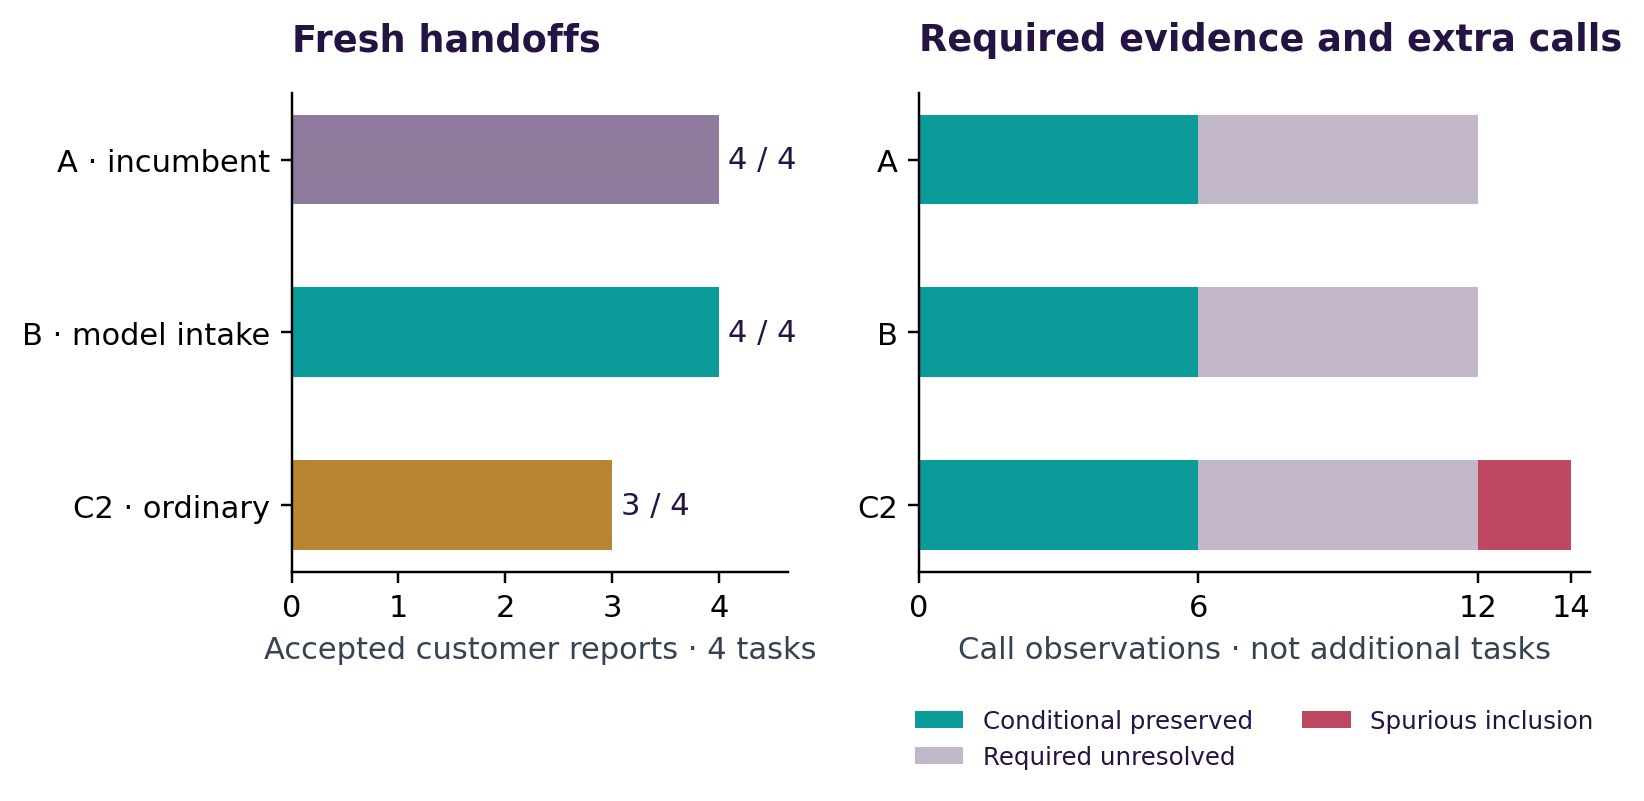
\includegraphics[width=\textwidth]{production-comparison.png}
\caption{Fresh customer-report acceptance and call-level evidence are different units. C2 covers the required calls but adds two out-of-scope data operations. The original failed primary remains a separate table and campaign.}
\end{figure}

The follow-up therefore demonstrates that prospective structured model intake can produce a source-bound customer review through the actual verifier. It does not identify a quality, operator-time or complete-cost gain over the incumbent. Its modest accuracy difference from this ordinary implementation is descriptive evidence on four purposive packages; it does not establish general superiority over competent conventional engineering.

A supplementary portability audit found a common integration defect outside the frozen customer-report checker: an auxiliary Workbench \texttt{fullTask} locator traversed one parent directory too few. All report links resolve and each exact raw task is attached, but the stronger claim that every original archive locator resolves is false for every arm. The sealed scores remain distinct from that finding. Publication assembly adds exact source aliases and records the repair separately without changing candidate code, output bytes or original acceptance. Complete source-license notices accompany the companion; standalone exports must retain the relevant notices.

The registered follow-up stopping rule is exhausted. C2 is not repaired against these answers, and the failed F03 task is not removed to create a favorable three-task cost comparison.


\section{Complete cost and the actual investment}
The cost account was opened before construction. Discovery already performed was listed as unpriced, not retroactively treated as free. The account includes literature and ownership discovery, both builders, rejected local snapshots, failed implementations, schema and runtime adapter corrections, verification, integration, the failed primary packages, fresh follow-up, simulation, reporting and future upkeep. Model authoring, extraction billing, provider tool charges, customer effort and some shared allocation remain unknown. These unknowns are part of the result.

We separate three quantities. \emph{Marginal process resources} are measured CPU, elapsed time and memory within recorded execution. \emph{Recurring complete cost} additionally includes input acquisition, extraction, verification, delivery, corrections and residual operator work for an accepted job. \emph{Fully loaded investment} includes the discovery, construction, failed candidates, integration and maintenance required for the exact retained asset. Measuring the first does not identify the other two. An asset construction cost is charged once, not both to investment and every mission.

Elapsed agent time is never multiplied by a human wage. The model/curator outputs are recorded artifacts, not necessarily one billable API request each. Stored-response replay measures deterministic continuation, not the latency or charge of generating a new response. C2's zero runtime model call count is an observed process distinction; its authoring and complete operating cost are not zero.

\subsection{Competent human delivery and break-even thresholds}
The official US Bureau of Labor Statistics reports May 2025 median annual pay of \$135,980 for software developers and \$104,300 for software QA analysts and testers \cite{bls}. Dividing by an explicitly assumed 2,080 hours gives wage anchors of \$65.375 and approximately \$50.144 per hour. These are employee wage anchors, not contractor quotes, loaded rates or measured durations for this work.

For a complete automated cost $c$ per accepted job and a matched human loaded rate $r$, the human-time break-even threshold is
\[
 t^* = \frac{60c}{r}\quad\text{minutes per equivalent accepted job}.
\]
For investment $I$, accepted workload $N$, incremental upkeep $M$ and per-job saving $s$, the elementary repayment condition is
\[
 Ns \ge I+M,\qquad N^* = \left\lceil\frac{I+M}{s}\right\rceil\quad(s>0).
\]
These thresholds are useful precisely because matched human durations are unknown. They do not claim that a maintainer takes any particular number of minutes or that every hypothetical job would be bought. If $s\le0$, this direct saving cannot repay a positive investment. In a strategic market, price response, rejection and timing can make the actual model threshold more demanding.

\begin{table}[htbp]
\centering\small
\begin{tabularx}{\textwidth}{Xlll}
\toprule
Quantity & A & B & C2\\
\midrule
Fresh customer reports accepted & 4/4 & 4/4 & 3/4\\
Recurring model/curator stage & Recorded & Recorded & None in execution\\
Complete recurring dollar cost & Unknown & Unknown & Unknown\\
Complete incremental construction & No new asset & Unknown & Unknown\\
Matched active customer/operator minutes & Unknown & Unknown & Unknown\\
Actual customer collections & \$0 & \$0 & \$0\\
\bottomrule
\end{tabularx}
\caption{The zero runtime model stage in C2 cannot earn an economic discount while complete equivalent work fails. Authoring a conventional program still incurs construction resources and unknown charges.}
\end{table}

The canonical shadow-ledger projection retains unknown total cost, profit and available operating surplus; it does not convert measured process resources into money. The final accounting snapshot gives one identity per recorded command, includes unsuccessful events, and preserves earlier snapshots and unknown discovery/authoring charges. The B and C2 asset manifests bind the actual tested entry points and source closures. Inactive comparison files included by provenance checks receive no productive credit.

For illustration only, a genuinely complete \$5 accepted job would break even against the developer wage anchor at approximately 4.59 active minutes, or against the QA wage anchor at 5.98 minutes. Neither the \$5 total nor those human durations was measured here. Likewise, a complete \$100 investment with a \$5 saving per equivalent accepted job and no upkeep would require twenty such jobs by simple arithmetic; those savings are not established for B or an accepted C2 replacement. The simulation must separately account for utilization, competition, failed work, maintenance, payment delays and foregone delivery.


\section{Connecting production to strategic buyer choice}
\subsection{A versioned extension of the existing simulator}
We extend the previous buyer-and-competitor simulator with a guarded, separately versioned adapter. The original source, protocols and histories remain unchanged. The extension supplies the exact tested asset identity, a complete construction envelope, active delivery cost and unchanged complete-workflow capacity. Default-path replays verify that the adaptation does not silently change historical behavior.

The market is a behavioral agent-based simulation, not a solved strategic equilibrium. Players are heterogeneous buyers, the focal enterprise, a human provider, conventional DIY/software and competing AI; doing nothing is available. Buyers differ in job value, budgets, required quality, effort, trust and switching costs. They choose among feasible offers, can reject or delay, and can leave a previously selected provider. Competitors adjust through the inherited price/quality/capacity/investment rules. These are declared policies, not Nash best responses proved optimal in this study.

Each week the model creates workload, updates alternatives and offers, evaluates buyer choices, executes only feasible jobs, accepts or rejects delivered work, posts invoices and bills, collects due payments, and considers an investment subject to cash and reserve constraints. Buyers know the modeled offer attributes and their own requirements; the enterprise forecasts from its observed history under the declared rule. Quality failures generate costs but not acceptance revenue. Capacity and budgets bind. A retained asset does not automatically create a sale.

For interpretation, a buyer's offer value can be represented schematically as
\[
 U_{ij,t}=\text{expected useful outcome}_{ij,t}-p_{j,t}
 -\text{effort}_{ij,t}-\text{switching}_{ij,t},
\]
subject to the actual implementation's budget, quality, trust and availability filters. The companion contains the exact functions; this expression explains the mechanism rather than replacing the executable model. We evaluate both the inherited deterministic and logit choice rules where calibration is uncertain.

The baseline scenario family uses 52 weeks, twelve buyers, finite \$1,000 initial cash, a \$200 reserve, \$50 setup, \$2 weekly overhead, two-week collection delay, and common quality, effort, trust and switching assumptions. These values are inherited or explicitly hypothetical inputs, not estimates established by our four fresh work packages. The new price policy is registered before its outcomes: a \$20 target, subject to the retained current-cost-plus-\$1 floor. Actual offers can therefore differ from the target. Lower-price stresses use \$5 and \$10 targets.

\subsection{What measured production may change}
Only independently equivalent complete work can enter the conditional cost comparison. The adapter rejects incomplete packages, scope-only acceptance, post-outcome favorable subsets, or an unproved model-stage distinction. A primary failed arm cannot be assigned a lower recurring cost merely because it did less work.

No executed evidence supports a B-specific increase in buyer value, quality, trust, capacity or lower integration effort. All such inputs remain common across arms. Local parsing time does not increase complete-workflow capacity. The model can test the conditional removal of a model/curator stage by C2 only if the fresh acceptance gate permits it. A/B receive the same uncertain charge for that stage; no asymmetric labor conversion is invented.

The registered campaign contains 24 no-benefit controls, 120 conditional cost/workload cells and 22 stress cells, each with eight paired seeds 3001--3008. The cost grid assumes a common \$5 nonmodel nominal delivery amount, an unknown A/B model-stage amount in \$0, \$0.25, \$1, \$5 or \$15, and complete construction envelopes of \$25, \$100 or \$500. Integration costs of \$0 or \$10 and arrival probabilities of 0.25 or 0.5 are crossed with the two buyer rules. These construction amounts are conditions, not measured totals or known upper bounds. All failed construction and uncertain shared allocation must fit within an envelope for that scenario to describe the real asset.

The stress slice is prespecified, not chosen after observing a winner. It covers stronger AI and price competition, human-provider response, low utilization, delayed collections, maintenance shocks and quality failure. Paired semantic draws preserve comparable opportunities across arms. The intervals reported by the simulator describe Monte Carlo variation conditional on assumptions; they do not quantify uncertainty about real demand or validate the choice model.

\subsection{Finance must occur at the decision time}
Let $C_t$ be cash, $R_t$ reserve, $O_t$ due obligations, and $E_t$ collected operating surplus available under the ledger's definition. An earned-financed investment requires both affordability and earned resources:
\[
 I_t\le C_t-R_t-O_t,\qquad I_t\le E_t.
\]
Receivables, initial capital, customer savings and token value cannot satisfy the second inequality by relabeling. The exact tested capability, its construction cost, integration pause, failures and maintenance are charged. A forecast of benefit is necessary but cannot override current funds. An unaffordable proposal must remain unbuilt.

The model reports enterprise profit, incremental value against the no-investment arm, investment repayment and available funds separately. Positive profit can come from the original service without justifying the new asset. Repayment is not the same as earning enough cash by the construction date. No second untested successor is inserted: \texttt{nextAsset} remains null. Thus even an earned-funded, repaid first asset is not evidence that a second worthwhile investment exists.

\subsection{Registered three-arm campaign: not admitted}
The complete four-job A/B/C2 gate fails because C2's F03 handoff fails. Consequently, \textbf{none of the planned 166 three-arm cells is executed}. The original grid and protocols remain unchanged. The three jobs that C2 passes are not substituted for the registered set, and its lack of a runtime model stage earns no financial discount. This is an economic admission failure grounded in delivered scope, not a requirement for actual sales.

\subsection{Separate accepted A/B diagnostic}
A new, explicitly exploratory diagnostic was registered after production and before its economic outcomes. It includes all four accepted A/B jobs, the same exact B asset and all 24 already prospective no-benefit stress cases with eight paired seeds. The original three-arm adapter is not weakened. A separate acceptance schema verifies every A/B job and independent audit row; C2 has no financial curve in this diagnostic.

Its prediction was stated before execution. When A and B have equal assumed complete nominal operating cost and no measured value, effort or capacity premium, incremental saving is zero. Positive construction cost, upkeep or interruption cannot create a positive repayment case. The model should refuse construction even if the underlying service occasionally earns a surplus. This prediction is algebraic; the executions test whether competition, cash timing, rejection and accounting respect it. They are not a new empirical estimate that B's true savings equal zero.

The campaign completes 192 paired worlds and 384 enterprise histories. A separate Python arithmetic audit reconciles every history without failure. It reconstructs 8,021 B decision-time earned-cash values and verifies that each investment consideration identifies the exact tested B asset. Every registered decision also lacks sufficient earned cash under the inherited reserve rule: the highest decision-time earned amount available is minus \$108. Thus both nonpositive incremental repayment and funding constraints bind in these histories; the observed refusals should not be attributed to only one of them. There are \textbf{zero constructions, zero earned-funded constructions and zero incremental B profit in every paired world}. Every operational A/B summary matches. The 2,066 delivery attempts are 1,033 per arm in paired copies, not independent real customers.

Twelve of 192 worlds per arm earn a positive modeled operating profit. Across all individual worlds, profit ranges from a loss of \$310 to a gain of \$86; every scenario's mean profit is negative. Positive service profit therefore does not justify the new asset. Its full bill is never charged as a completed modeled construction because no investment proceeds; the actual research construction that produced it occurred outside the simulation and remains explicitly unpriced in the historical account. Those modeled receipts did not finance this research.

\begin{table}[htbp]
\centering\small
\begin{tabularx}{\textwidth}{Xrrrr}
\toprule
Stress & \multicolumn{2}{c}{Mean profit (USD)} & \multicolumn{2}{c}{Mean accepted}\\
 & Determ. & Logit & Determ. & Logit\\
\midrule
Reference & -154.00 & -40.25 & 0.000 & 7.875\\
Zero demand & -154.00 & -154.00 & 0.000 & 0.000\\
Low demand & -154.00 & -107.12 & 0.000 & 3.125\\
Target \$10 & -116.19 & -96.81 & 10.750 & 13.500\\
Target \$5; floor \$6 & -149.50 & -144.38 & 22.875 & 20.625\\
Stronger, cheaper AI & -154.00 & -146.50 & 0.000 & 0.500\\
Cheaper human provider & -154.00 & -66.50 & 0.000 & 6.000\\
Competitor price response & -104.94 & -11.19 & 3.500 & 10.125\\
Delayed collections & -154.00 & -50.25 & 0.000 & 7.875\\
Quality failures & -145.88 & -93.06 & 1.250 & 5.000\\
Maintenance shock & -154.00 & -40.25 & 0.000 & 7.875\\
Cash and capacity stress & -310.00 & -306.88 & 0.000 & 0.625\\
\bottomrule
\end{tabularx}
\caption{All twelve diagnostic stresses, eight seeds per buyer rule. A and B have identical outcomes, zero investments and unknown actual monetary cost. Simulated accepted counts are not observed customer jobs.}
\end{table}


\begin{figure}[htbp]
\centering
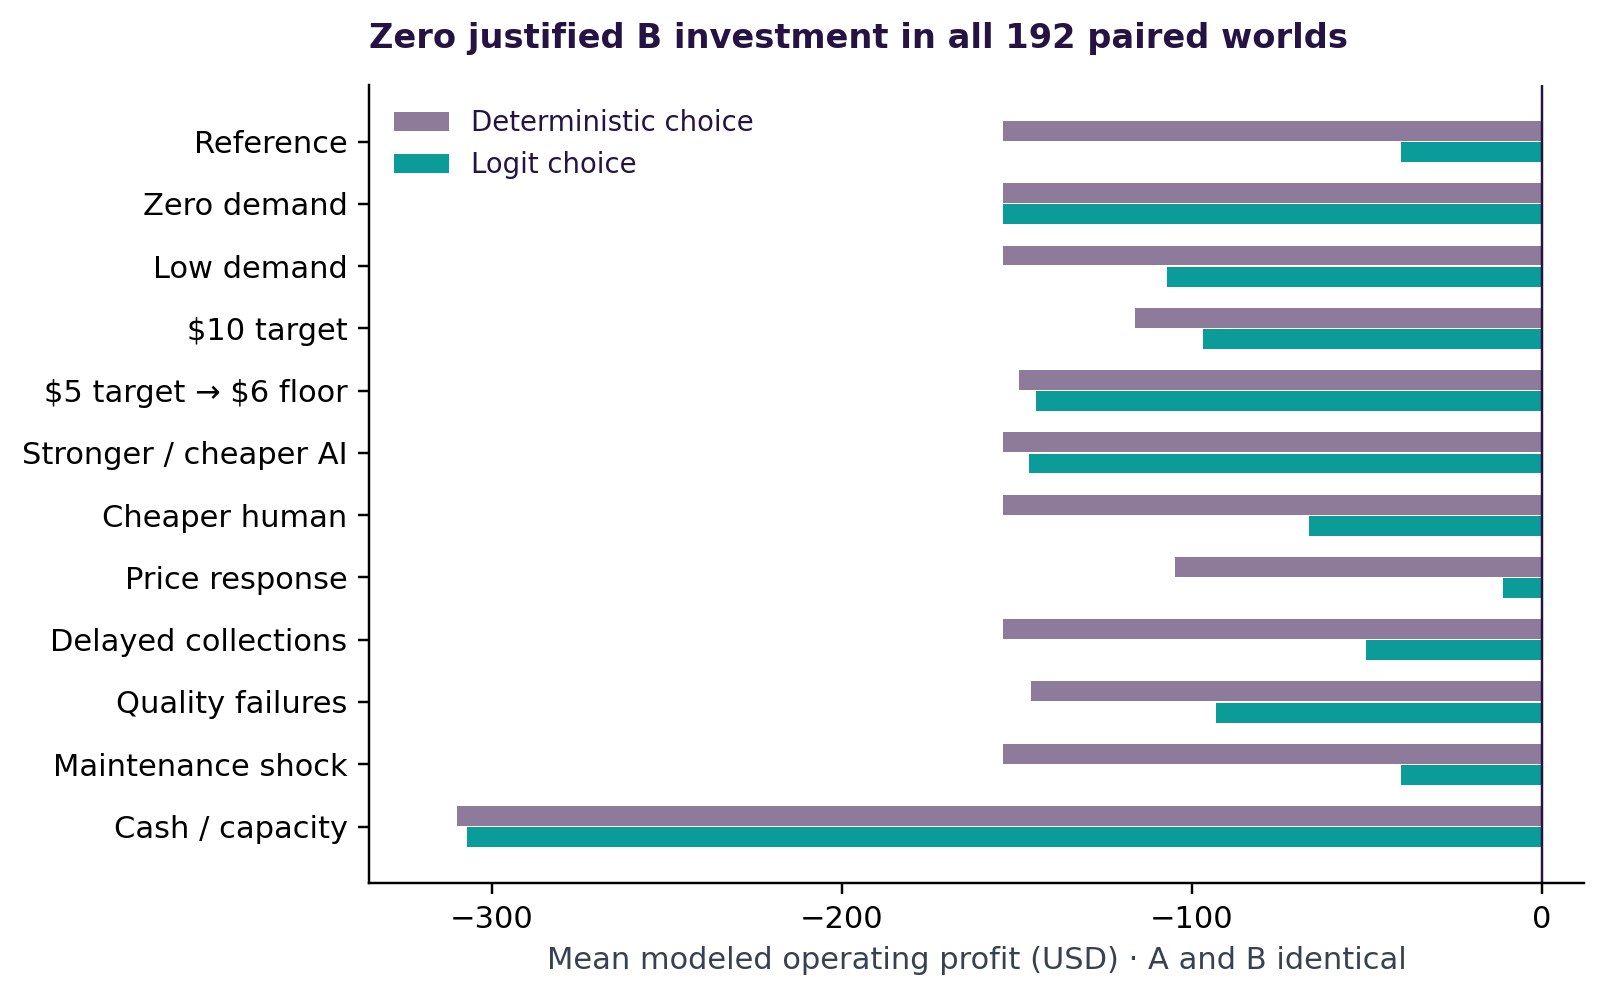
\includegraphics[width=\textwidth]{market-diagnostic.png}
\caption{Mean operating profit under both buyer-choice rules for every registered A/B diagnostic stress. A and B coincide in all paired worlds. These conditional outputs are not demand estimates; no scenario mean is profitable and no B investment proceeds.}
\end{figure}

The reference deterministic rule buys no enterprise output and incurs \$154 in setup and weekly overhead. The reference logit rule averages 7.875 accepted deliveries and a \$40.25 loss, with two profitable worlds. Alternative buyer modeling therefore changes allocation and service viability without producing a capability-investment case. A \$10 target produces more accepted work but insufficient mean margin. The \$5 target is actually floored at \$6 by the retained nominal-cost-plus-\$1 policy; its higher volume still does not recover overhead on average.

Stronger low-cost AI sharply reduces the logit enterprise's accepted volume. Delayed collections separate accounting profit from available cash. The combined cash/capacity stress leaves a maximum modeled loss of \$310 and retained obligations, rather than permitting unaffordable construction. A maintenance shock has no realized asset-maintenance bill when no asset is built; it still cannot make the refused investment worthwhile. All stress outcomes, actual offer histories and refusal reasons are retained, including profitable seed draws and unfavorable cases. All sixteen insolvent case-seed combinations per arm occur in the combined cash/capacity stress. The highest-profit world earns \$86 but retains minus \$114 in the model's earned-surplus measure after its \$200 reserve; its \$1,086 total cash still includes \$1,000 initial capital.

There is no finite break-even workload for B \emph{through the asserted zero-saving mechanism}: repetition multiplies zero incremental saving. This is conditional on the diagnostic's common-cost assumption, not a universal statement about the real asset. Reversing the investment conclusion requires a substantiated incremental complete-cost reduction, useful quality/value gain, or complete-workflow capacity improvement, together with sufficiently recurring demand and decision-time cash. Lowering B-specific switching or trust costs without evidence is not such a substantiation.

\paragraph{Additional incentive-path software control.}
Because every registered decision also lacks earned funding, a separately labeled post-campaign control tests refusal when cash is sufficient. Its declared single seed is 3001; common integration and reserve are zero, arrival probability is one, the common nominal cost is \$5, price target \$20, and the exact B construction envelope \$25. Other quality and competitor settings remain unchanged. All 44 decision weeks are cash-eligible and still refuse construction. At week eight, earned funds are \$162 against the \$25 bill, but incremental saving remains zero and expected net benefit is negative. This control adds no registered market cell or demand evidence; it tests the incentive branch without the cash constraint. Its positive common-service profit must not be pooled with the registered stress campaign or represented as a financed B improvement.


\section{Robustness, uncertainty and failure conditions}
Several limitations are structural. Public historical source tasks are not paid jobs. Their recurrence and prevalence do not identify a weekly arrival rate. A maintainer may receive sufficient value from free tooling and existing tests; the residual call review may be too narrow to command the modeled price. Source-level binding does not establish correct behavior. A conservative HOLD can be useful, but its customer value depends on how much uncertainty it actually removes.

Cost identification is equally important. The exact historical authoring bill cannot be recovered from local CPU receipts. A cheap deterministic process may be expensive to construct and maintain. If the full cost lies above a scenario envelope, that cell cannot support the actual investment. If common verification or customer integration dominates, eliminating extraction may not materially change the complete cost. Capacity improvements are unsupported without a full delivery and operator-time study.

The independent oracle reduces one kind of circularity but does not eliminate all dependence. Roles share a session, host and language-model family. Source selection is purposive, and two primary transitions reuse one component. The follow-up is intentionally separate and small; it is not pooled with the failed primary to manufacture a larger success rate. The revised comparator reflects a general defect discovered in primary evaluation, so only new held-out sources qualify as fresh evidence for it.

The financial model is accounting-validated and incentive-tested, not demand-validated. Its heterogeneous buyers, rejection option and competitor responses prevent several easy false positives, but do not make hypothetical preferences empirical. Different plausible preference and switching models can reverse adoption. Eight paired seeds stabilize descriptions within a cell; more seeds would not solve uncertain structural assumptions. We stop at the registered campaign rather than repeatedly tuning on its outputs.

\section{Implications for the AGI ALPHA Flywheel}
Transformational Intelligence is operationalized here as a search for structural changes that remove recurring work or make reliable verification cheaper. The strong alternative is therefore essential. If reusable ordinary extraction can satisfy the same bounded acceptance, the next investment should be evaluated as that exact asset; a research label cannot claim the saving. Conversely, unsupported dynamic source relationships remain a legitimate place for careful model-assisted investigation, provided its complete cost and incremental value are measured.

The practical contribution is an executable discipline: freeze the real incumbent and candidate; deliver a useful bounded outcome; audit completeness and handoff independently; charge failed construction; carry only measured differences into a strategic model; and require the ledger to fund the same tested asset. This discipline produced preserved negative evidence as well as working artifacts. It does not require actual sales to conduct a credible simulation, and it does not permit a simulation to stand in for actual collections.

\textbf{Decision.} Retain the source-intake implementation and its evidence as a research capability, but do not claim that the DUPLEX-inspired intervention has earned a financially justified production expansion. It executes fresh bounded reviews and matches the incumbent's accepted conclusions. Its complete monetary and effort advantage is unidentified. C2 remains a preserved, partly successful conventional alternative whose failed complete scope blocks the planned model-free savings comparison.

The evidence supports a functional adaptation of structured extraction and exact verification. It does not reproduce the external planning results, establish a distinctive economic advantage, finance another worthwhile tested capability, or demonstrate self-acceleration. OpenEvolve and EnvHarness were reviewed and deliberately not installed or claimed as evaluated. The previous primary negative market result remains intact; the new exploratory A/B diagnostic confirms only the narrower financing and accounting constraint registered for it.

A modeled commercial Flywheel is not established, and a realized one is not established. No paid pilot was required to reach those conclusions. The binding next evidence is complete incremental cost and effort for equivalent accepted delivery, a conventional workflow with complete scope, and defensible recurrence and buyer calibration. Until those observations exist, retaining cash and declining an unsupported construction is the rational modeled action.


\appendix
\section{Reproduction and evidence map}
The companion's README gives exact commands and source identities. Production replay consumes the stored prospective extraction/curator responses and runs the unchanged Workbench and product core. That replay reproduces the deterministic continuation, not an independent new draw from an externally billed model. The independent acceptance programs parse the original captured source and check complete packages. The market runner refuses a changed source closure or an existing result destination; its auditor reconciles each history independently.

\begin{longtable}{p{47mm}p{107mm}}
\toprule
Artifact group & Purpose and boundary\\
\midrule\endhead
\artifact{protocol/} & Original and follow-up protocols, candidate/input/execution freezes and frozen model prompt.\\
\artifact{vendor/} & Exact public product and native Workbench closures with source manifests and original licenses.\\
\artifact{inputs/}, \artifact{transcripts/} & Captured public tasks, raw model/curator artifacts and extraction provenance.\\
\artifact{acceptance/}, \artifact{acceptance-followup/} & Independently selected sources, oracle, protocol, controls and license records; original identities preserved.\\
\artifact{results/} & Every scheduled outcome, Workbench pack, receipts and separate primary/follow-up audits.\\
\artifact{resources/} & Process instrumentation and complete-cost register, including unknowns and unsuccessful attempts.\\
\artifact{market/} & Unchanged inherited source, derived adapter, prospective grid, full new histories, cash ledgers and independent audits.\\
\artifact{publication/} & LaTeX, figures, PDF, bilingual offline demonstration and build/QA evidence.\\
\bottomrule
\end{longtable}

Prior original market archives remain identified by immutable SHA-256 in the audit register. Their authors' publications and release lanes are not overwritten by this contribution. The repository contribution is additive and source-only. Local tests and artifact checks do not replace hosted repository qualification, full installation, security review or operator authorization.

\section{Licenses, provenance and interpretation}
New integration source carries Apache-2.0 identifiers. The vendored Alpha and Jobs source notices and captured third-party notices remain attached. Open-source license permission does not imply endorsement. ArXiv version identifiers and repository commit identities, not floating project names alone, define the inspected literature. The personal creator--critic--verifier document is referenced by its local provenance record without redistributing its content.

Measured values, sourced external inputs and hypothetical scenarios are presented distinctly in the paper and demonstration. Actual collections equal zero. A full-cost unknown is neither zero nor a measured bound. ``Accepted'' in a source audit means the stated bounded engineering deliverable passed its independent criteria; it does not mean a buyer purchased it or approved a deployment.

\begin{thebibliography}{12}
\bibitem{coordination} MontrealAI. AGI ALPHA coordination issue 4850 and linked source/publication lanes. \url{https://github.com/MontrealAI/AGI-Alpha-Agent-v0/issues/4850}. Inspected 26 October 2026.
\bibitem{vae} N. Toma\v{s}ev, M. Franklin, J. Z. Leibo, J. Jacobs, W. A. Cunningham, I. Gabriel, and S. Osindero. \emph{Virtual Agent Economies}. arXiv:2509.10147v1, 12 September 2025. \url{https://arxiv.org/abs/2509.10147v1}.
\bibitem{duplex} K. Hua, D. Wang, Y. Gu, and X. Ma. \emph{DUPLEX: Agentic Dual-System Planning via LLM-Driven Information Extraction}. arXiv:2603.23909v1, 25 March 2026. \url{https://arxiv.org/abs/2603.23909v1}.
\bibitem{openevolve} Algorithmic Superintelligence. \emph{OpenEvolve}, source at \path{66856ac4ba2f51382c26ca210361db4deb69b9d9}, package 0.4.0. \url{https://github.com/algorithmicsuperintelligence/openevolve}.
\bibitem{envharness} C. Huang et al. \emph{EnvHarness: Awakening Static Worlds for Agent Learning}. arXiv:2608.19880v1, 20 August 2026; Google Research implementation at \path{fab7d57441f06b75c73a900e04561d4d7600f361}. \url{https://arxiv.org/abs/2608.19880v1}; \url{https://github.com/google-research/envharness}.
\bibitem{dependabot} GitHub. \emph{Dependabot version updates}. Official documentation, inspected 26 October 2026. \url{https://docs.github.com/en/code-security/concepts/supply-chain-security/dependabot-version-updates}.
\bibitem{renovate} Mend. \emph{Mend Renovate Cloud resource tiers}. Official documentation, inspected 26 October 2026. \url{https://docs.mend.io/renovate/latest/mend-renovate-cloud-resource-tiers}.
\bibitem{bls} US Bureau of Labor Statistics. \emph{Software developers, quality assurance analysts, and testers}, Occupational Outlook Handbook, May 2025 pay figures. \url{https://www.bls.gov/ooh/computer-and-information-technology/software-developers.htm}. Inspected 26 October 2026.
\end{thebibliography}
\end{document}
